
\section{Evaluation}
\label{sec-sck-eval}


We now evaluate our \sck integration to Cassandra. Our evaluation answers the
following questions.
%
\sec\ref{eval-accu}: How accurate is \sck compared to real deployments?
%
\sec\ref{eval-bugs}: Can \sck find old scalability bugs?
%
\sec\ref{eval-new}: Can \sck reveal new bugs?
%
% \sec\ref{eval-mem}: How long is the output and time memoization overhead?
%
\sec\ref{eval-other}: Does our evaluation compare well with other work?


We use the Nome cluster; each machine has 16-core AMD Opteron(tm) 8454
processors with 32-GB DRAM \cite{NomeNodes}.
%
To measure \sck accuracy (\sec\ref{eval-accu}), we compare it with real
deployments of 32, 64, 128, 256, and 512 nodes, deployed on at most 128 Nome
machines.\footnote{The Nome cluster only has 256 nodes and near the publication
deadline, we need to fair-share the cluster with other groups.  Our target
protocols only make at most 2 busy cores per node, which justifies why we run 8
nodes per one 16-core machine for the real deployment.}
%

\subsection{Accuracy}
\label{eval-accu}

\def \fff        {$f$}
\def \flaps      {\textit{\#flaps}\xspace}
\def \gosLast    {$T_{lastGossip}$\xspace}
\def \gosAvg     {$T_{avgGossip}$\xspace}
\def \gosProc    {$T_{gossipExec}$\xspace}
\def \supProc    {$T_{stateUpdate}$\xspace}
\def \hops       {\textit{\#hops}\xspace}

\def \ringTable  {$Size_{ringTable}$\xspace}
\def \newStates  {$Size_{newStates}$\xspace}
\def \cpuSpeed   {$CPU$\xspace}


Next, we provide a detailed accuracy evaluation of \sck.  Due to space
constraints, this section only focuses on one bug (\caone \cite{CA-One}) 
while the next
section briefly discuss other bugs we reproduced.




% metrics
Figure \ref{fig-form}a-d presents the  internal metrics within
Cassandra failure detection protocol that we measured for {\em every pair}
of nodes.  That is, the algorithm runs on every node A for every peer B.
%
Figure \ref{fig-accu}a-d compare in detail the accuracy of \sck compared
to real deployments.
%
For example, $x$$=$512 implies the comparison of 512-node colocation in
\sck versus a real deployment of 512 nodes.
%
Note that for \caone, we only need time profiling with offline sampling
(\sec\ref{sc-pil-4}) and no pre-memoized data (\sec\ref{sc-pil-3}).  
%


% ------------------------ a
Figure \ref{fig-accu}a shows the total number of flaps (alive-to-dead
transitions) observed in the whole cluster during bootstrapping.  
As shown, \sck closely mimics
real deployment scenarios.  Most importantly here, a significant \flaps
does not appear until 256-node deployment, 
hence mini-cluster extrapolation techniques will not work (\sec\ref{mot-state}).
%
Figure \ref{fig-form}a defines that \flaps depends on 
\phi \cite{Hayashibara+04-PhiFailureDetector}.  Every node A
maintains a \phi value for a peer node B (a total of $N$$\times$$(N$$-$$1)$
variables to monitor).  If \phi$>$8 for B, A will declare B dead (a flap).

% ------------------------ b
Figure \ref{fig-accu}b shows the maximum \phi values observed for every
peer node.  For example, for the 512-node setup, the whisker plots show the
distribution of the maximum \phi values observed for each of the 512
nodes.  As shown, the larger the cluster, more \phi values exceeds the
threshold value of 8, hence the flapping.
%
Figure \ref{fig-form}b points that \phi depends on the average
inter-arrival time of when new gossips about B arrives at A (\gosAvg) and the
time since A heard the last gossip about B (\gosLast); the ``last gossip''
is the last version number received (\sec\ref{mot-bug}).  The point is that
\gosLast should not be much higher than \gosAvg.




% d) $T_{avghbperiod}$ = h(all previous $T_{hbsilence}$) \\



\def \fgap {~~~~~~~~~~}
\def \fgap {~~~~}


\begin{figure}

\small
\centering


\begin{spacing}{1.5}
\begin{tabular}{|p{3.2in}|}
\hline

a) \flaps = \fff $($ \phi $>$ $8$ $)$ \\

b) \phi = \fff $($ \gosAvg, \gosLast $)$ \\
\fgap   \gosAvg = avg. of last 1000 \gosLast \\

c) \gosLast = \fff $($ \hops, \gosProc $)$ \\
\fgap \hops = $log(N)$ on average \\
\fgap \gosProc = \supProc (if new state changes) \\

d) \supProc = \fff $($ \ringTable, \newStates $)$ \\

\fgap   \ringTable $\leq$ $N$$\times$$P$ and \newStates $\leq$ $N$ \\



\hline
\end{tabular}
\end{spacing}

\vfive % orphan : we have extra space on page 10

\mycaption{fig-form}{Cassandra internal metrics (\sec\ref{eval-accu})}{Above
are the metrics we measured within the Cassandra bootstrap protocol
for measuring \sck accuracy (Figure \ref{fig-accu}). 
``f'' represents ``a function of'' (\ie, an arbitrary function).}


\end{figure}





% ------------------------ c
Figure \ref{fig-accu}c shows the whisker plots of gossip inter-arrival
times (\gosLast) that we collected for every A-B pair.  For example, for the
512-node setup, the whisker plots represent the distribution of 
around 41 million 
gossip inter-arrival times; this large number is because a message
contains gossips of many peer nodes.  The figure shows that in larger
clusters, new gossips do not arrive as fast as in smaller clusters,
especially at high percentiles.
%
Figure \ref{fig-form}c shows that \gosLast depends on how far B's new
gossips propagate through other nodes to A (\hops) and the gossip
processing time in each hop (\gosProc).  The \hops is stable
at $log(N)$ on average in \sck and real deployment (not shown).  The
latter (\gosProc) is essentially state-update processing time (\supProc)
whenever there are state changes, which is the culprit.

% ------------------------ d
Figure \ref{fig-accu}d ({\em in log scale}) shows the whisker plots of
state-update processing time (\supProc); in the 512-node setup, we
measured around 25,000 state-update invocations.  The figure shows that at high
percentiles, \supProc is scale-dependent.  As explained in 
Figure \ref{fig-form}d (and Section \ref{mot-bug}), \supProc complicatedly
depends on a scale-dependent 2-dimensional input (\ringTable and
\newStates); a node's \ringTable depends on how many nodes it knows,
including the partition arrangement ($\leq$$N$$\times$$P$) and \newStates
($\leq$$N$) increases as cluster size increases.
%
%The bug was not expected because the median of \supProc is not
%scale-dependent.
%
Note that the \supProc in \sck comes from the sampling-based time
profiling (\sec\ref{sc-pil-4}), which is relatively accurate as the figure
shows.




\def \fgw {2.7in}



\begin{figure}[t]

%\centerline{

%}



\centerline{
%\hmina
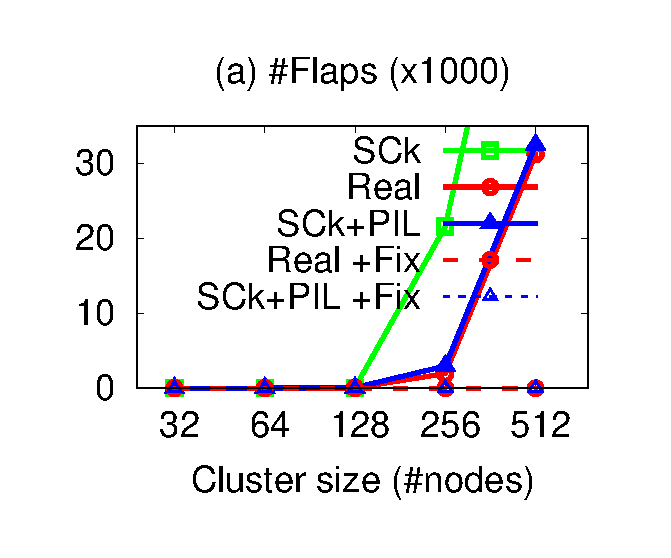
\includegraphics[width=\fgw]{F/accu/eps/flap}
%\hminb
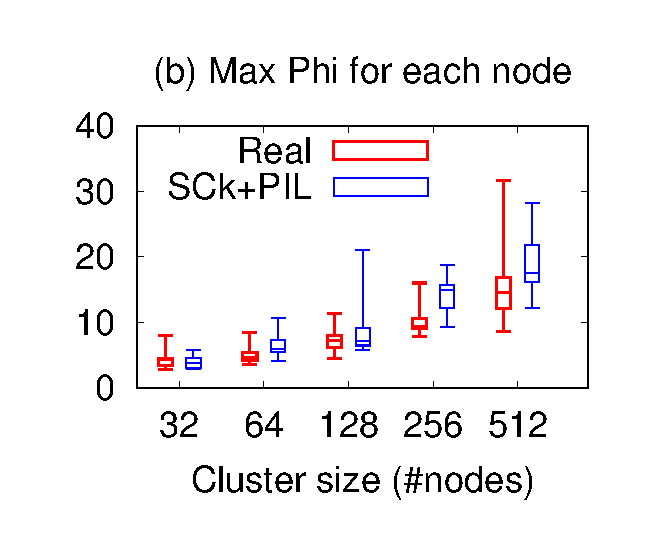
\includegraphics[width=\fgw]{F/accu/eps/phi}
%\hmina
%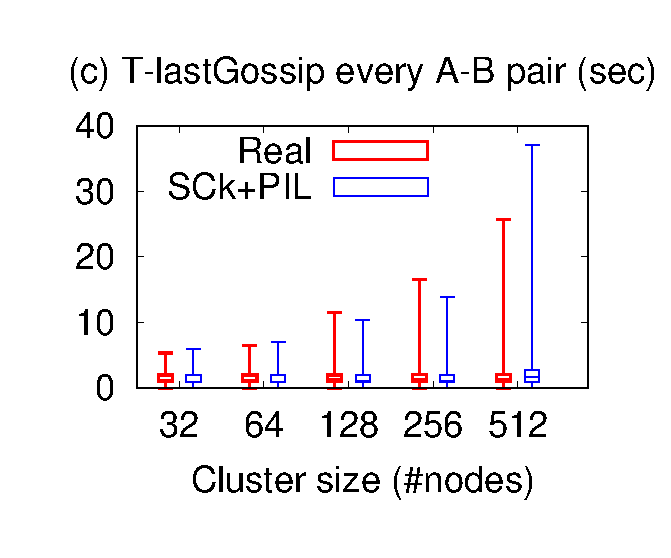
\includegraphics[width=\fgw]{F/accu/eps/hb}
%\hminb
%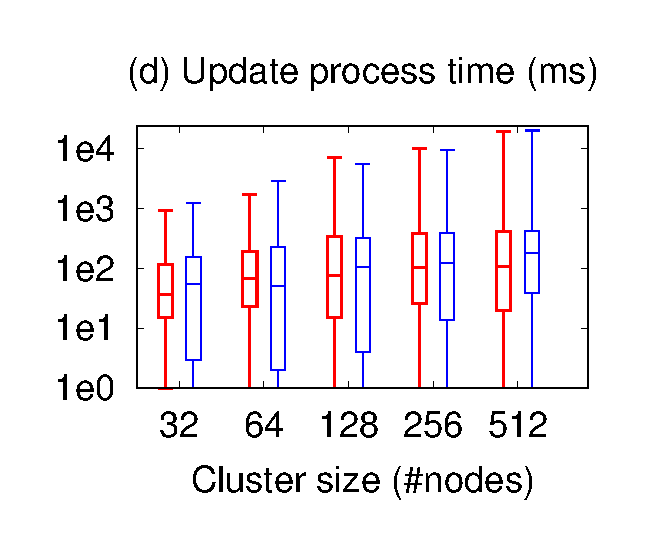
\includegraphics[width=\fgw]{F/accu/eps/proc-log}
}

%\vfive % orphan : we have extra space on page 10

\centerline{
%\hmina
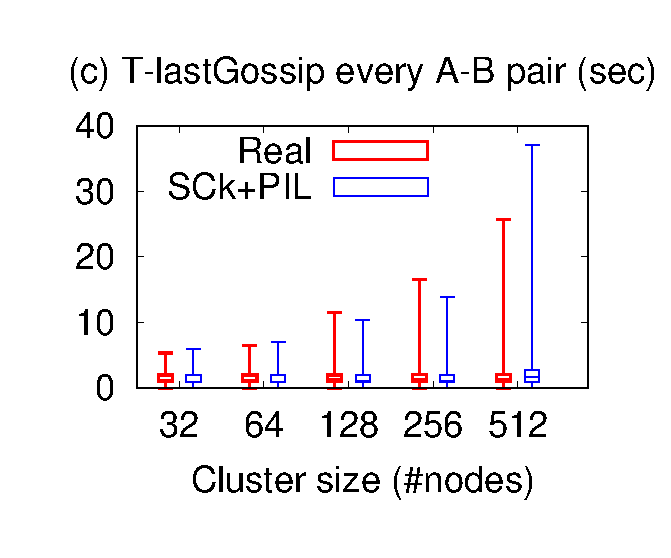
\includegraphics[width=\fgw]{F/accu/eps/hb}
%\hminb
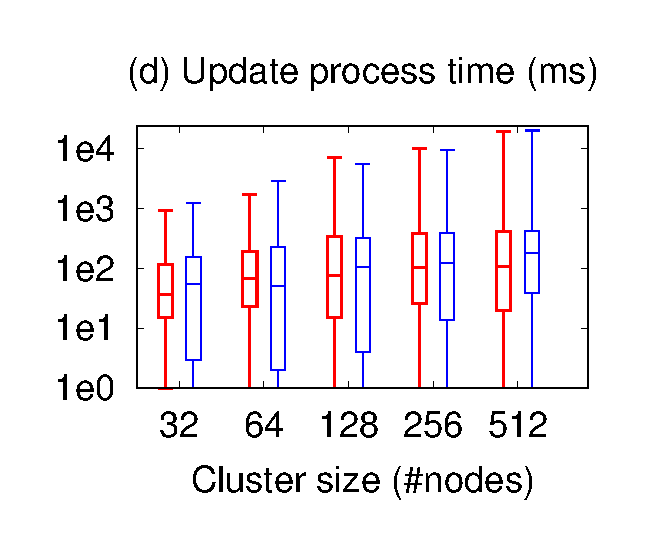
\includegraphics[width=\fgw]{F/accu/eps/proc-log}
}

%\centerline{
%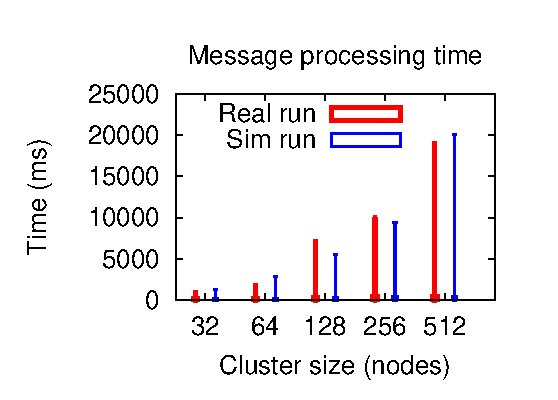
\includegraphics[width=\fgw]{F/accu/eps/proc}
%\includegraphics[width=\fgw]{F/accu/eps/hop}
%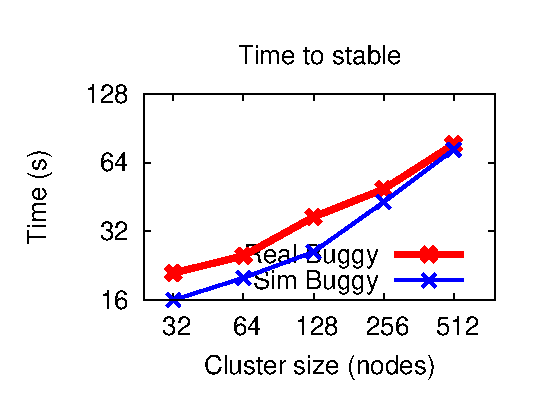
\includegraphics[width=\fgw]{F/accu/eps/stable}
%}

\vminten
\mycaption{fig-accu}{Accuracy in reproducing \caone (\sec\ref{eval-accu})}{The 
figures represent the metrics presented in Figure \ref{fig-form},
measured in real deployment (``Real'') and \sck with
different cluster sizes (32, 64, 128, 256, and 512).
Figure title represents the y-axis.}
\vminfive
\end{figure}




\if 0

\hsg{ b - 512
 c - 41295431
 d - 24335
recap, exampe, how many data points.
}

% \includegraphics[width=\fgw]{F/graphs/ca-6127/tsilent_99}
% \includegraphics[width=\fgw]{F/graphs/ca-6127/avgtsilent_99}
\includegraphics[width=\fgw]{F/graphs/ca-6127/avgtsilent}
\includegraphics[width=\fgw]{F/graphs/ca-6127/hop}
\includegraphics[width=\fgw]{F/graphs/ca-6127/hop}
\includegraphics[width=\fgw]{F/graphs/ca-6127/proctime}
\includegraphics[width=\fgw]{F/graphs/ca-6127/proctime_99}
\includegraphics[width=\fgw]{F/graphs/ca-6127/commit}
\includegraphics[width=\fgw]{F/graphs/ca-6127/commit_99}
\includegraphics[width=\fgw]{F/graphs/ca-6127/profiling}
\includegraphics[width=\fgw]{F/graphs/ca-6127/table}
\includegraphics[width=\fgw]{F/graphs/ca-6127/table_med}
\fi



We conclude that \sck mimics similar behaviors as in real deployments and
is accurate for reproducing scalability bugs.
%
As an additional note, we have applied the bug patch in both \sck and real
deployment modes;  Figure \ref{fig-accu}a shows \flaps is always zero in
both modes.



\subsection{Bugs Reproduced}
\label{eval-bugs}



Table \ref{tab-bugs} lists all the \numEval bugs\footnote{Given the limited
time and number of students.}   we have reproduced (4
Cassandra, 1 Riak, and 1 Voldemort bugs).
We chose these \numEval bugs
(among the \numStudy bugs we studied) because the reports contain 
more detailed
descriptions about the bugs, the affected protocols, the affected code
version numbers, configuration setups, and the patches.  Table
\ref{tab-bugs} also shows the number of nodes needed for the bug symptoms
to surface and the quantifiable metrics of the symptoms.
%
Our first target system was Cassandra, hence the more bugs reproduced
compared to Riak and Voldemort; the latter two were added for  stronger
proof of concept.
%
Figure \ref{fig-bugs} shows the accuracy of \sck in reproducing the 6 bugs
using the metrics shown in Table \ref{tab-bugs}.
%
The first bug, \caone, has been described in \sec\ref{mot-bug} and
\sec\ref{eval-accu}.
%
We now briefly discuss the other five bugs 
(shown in Figure \ref{fig-bugs}) and then
%
make several important remarks.


Figure \ref{fig-bugs}a: In \catwo \cite{CA-Two}, 
when a node D is decommissioned from a
large cluster, all other nodes must own D's key-partitions.
This scale-dependent ``pending keyrange calculation'' is CPU intensive,
causing cluster-wide flapping, significantly observable in 256+ nodes.
The developers fixed it by caching outputs of slow methods.

Figure \ref{fig-bugs}b: \catri \cite{CA-Tri} 
is similar to the previous bug (\catwo),
but the fix was not efficient enough because in this new bug, the concept
of ``virtual nodes'' (multiple key-partitions per node) was added to
Cassandra.  The calculation is now scale-dependent to $N$$\times$$P$ and
becomes very CPU intensive.  This causes massive flapping during scaling out; 
the bug surfaced in 64+ nodes (when 32+ new nodes are added
to existing 32+ nodes). The bug was fixed with a complete 
redesign of the pending keyrange calculation.
%



\begin{table}
\begin{center}
\small
\centering
%---------------------------------
\begin{tabular}{l|r|l|l} 
{\bf Bug\#} & 
{\bf Surface} & 
{\bf Protocol} & {\bf Metric} \\
\hline
\caone \cite{CA-One} &$N$$\geq$256 & Bootstrap & \flaps \\
\catwo \cite{CA-Two}   & $\geq$256 & Decommission & \flaps \\
\catri \cite{CA-Tri}   & $\geq$64 & Add new nodes & \flaps \\
\cafour \cite{CA-Four}  & $\geq$256 & Add new nodes & \flaps \\
\riakone \cite{RIAK-One} & $\geq$128 & Boot+rebalance & $T_{Complete}$ \\
\voldone \cite{VOLD-One} & $\geq$128 & Rebalance & $T_{Complete} $ \\
\end{tabular}
%---------------------------------
\end{center}
\vminten
\mycaption{tab-bugs}{Reproduced bugs (\sec\ref{eval-bugs})}{``Surface'' 
implies the number of nodes
needed for the bug symptom to surface.
``c'' stands for Cassandra, ``r'' for Riak, and ``v'' for
Voldemort. 
}
\vminfive
\end{table}





Figure \ref{fig-bugs}c: Interestingly, \cafour \cite{CA-Four} is 
a bug in the {\em same}
protocol as in the previous bug.  We wondered why the previous fix does
not work here.  We found that pending range calculation is now
multi-threaded; different range calculations can happen concurrently.
This new design however introduces a new coarse-grained lock that creates
a new problem;  it can block gossip processing for a long
time, thus introduce flapping (in 256+ nodes).  The fix changed the
lock management.
%
The figure also shows that, for this workload, offline time profiling
is not fully accurate as the bug is order sensitive at large scale.
We are now testing it with order determinism. 


Figure \ref{fig-bugs}d: In \voldone \cite{VOLD-One}, 
Voldemort's rebalancing was not
optimized for large clusters; it led to more stealer-donor partition
transitions as the cluster size grows (128+ nodes).  To fix this, the
developers completely changed the stealer-donor partition 
transition algorithm.


Figure \ref{fig-bugs}e: In \riakone \cite{RIAK-One}, Riak bootstrapping
employed a complex 3-stage rebalancing algorithm (claim-target,
claim-hole, full-rebalance) that each node runs to eventually converge and
achieve a  perfect balance of the ring.  Each node runs this
CPU-intensive algorithm on {\em every} bootstrap gossip received.  The
larger the cluster, the longer time perfect balance is achieved (observed in
128+ nodes).
% This decentralized
% rebalancing was fixed with a centralized rebalancing.  
For Riak, we profile the rebalancing time along with pre-memoization (with
order determinism; \sec\ref{sc-pil-3}-\ref{sc-pil-4}).  Figure
\ref{fig-bugs}f (similar to Figure \ref{fig-accu}d) compares the execution
time of the rebalance function invocations in \sck and real deployments.
The figure shows that \sck's PIL exhibits a high accuracy.




\def \fgw {1.77in}


\begin{figure}[t]

\vminten

\centerline{
\hmina
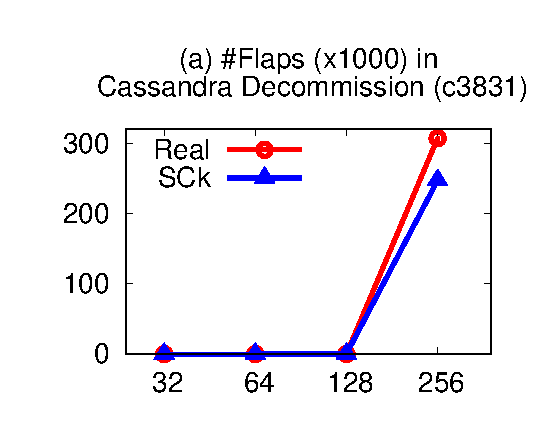
\includegraphics[width=\fgw]{F/old-bugs/eps/cass2.eps}
\hminb
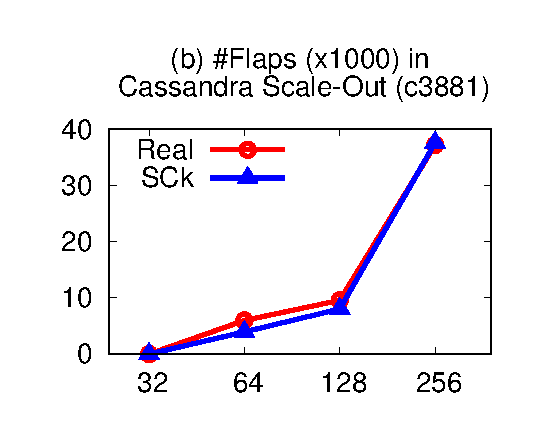
\includegraphics[width=\fgw]{F/old-bugs/eps/cass3.eps}
\hmina
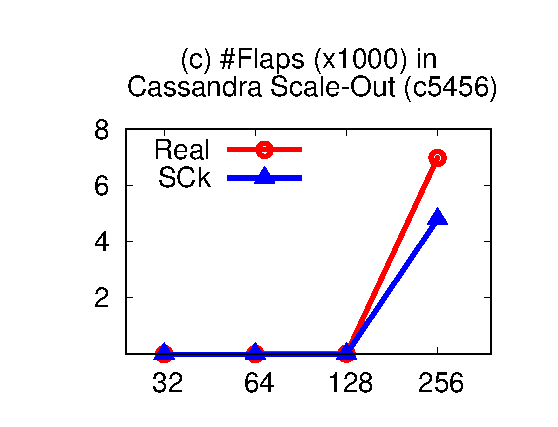
\includegraphics[width=\fgw]{F/old-bugs/eps/cass4.eps}
}
%\centerline{
%\hmina
%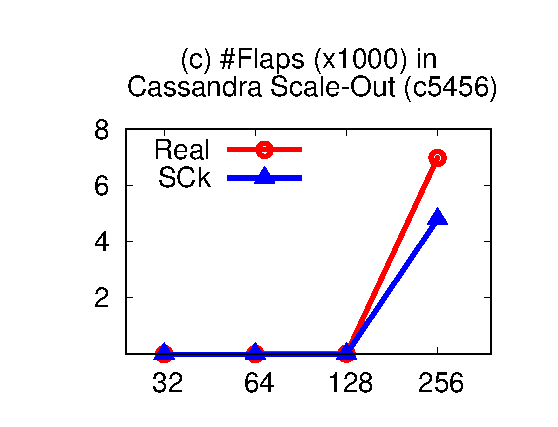
\includegraphics[width=\fgw]{F/old-bugs/eps/cass4.eps}
%\hminb
%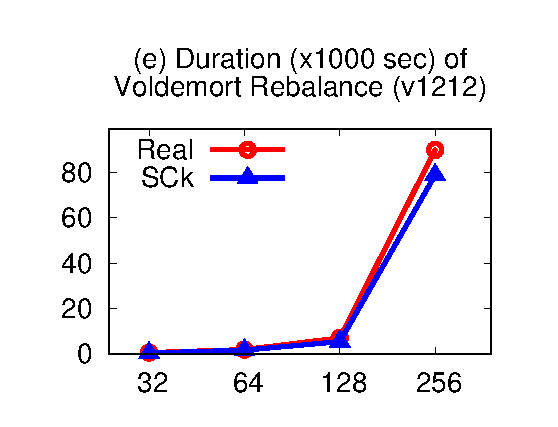
\includegraphics[width=\fgw]{F/old-bugs/eps/vold1.eps}
%}

%\centerline{
%\hmina
%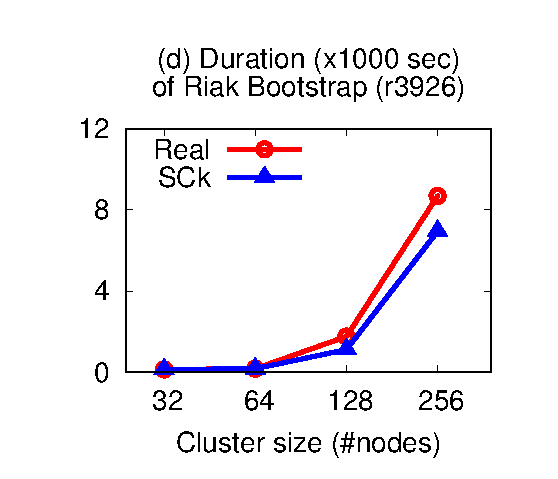
\includegraphics[width=\fgw]{F/old-bugs/eps/riak1.eps}
%\hminb
%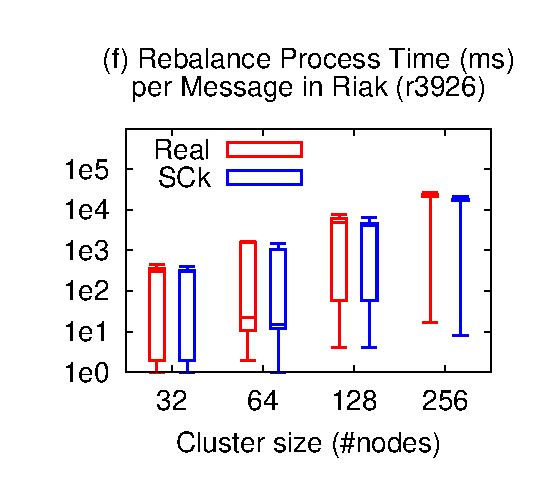
\includegraphics[width=\fgw]{F/riak/eps/proc.eps}
%}

\vminfive

\mycaption{fig-bugs}{Accuracy in reproducing other 
bugs (\sec\ref{eval-bugs})}{The
figures represent the bugs described in Table \ref{tab-bugs}.  
The title represents the y-axis. 
We cap the y-axis to show the scale at which the bug symptoms start
to appear. }
\vminfive
\end{figure}



\if 0

TODO: CASS2: waiting for NOme to go up.
Meanwhile doing CASS3. 
%
RIAK: Buggy done, but need to plug in data from new version
(Cesar is adding fixed/patched line from the newest version).
%
VOLD: (Wait until all features are in).  Still running.
\fi




We make several remarks from this experience.
%
First, if \sck had existed in the first place, it might have {\em
  prevented} the Cassandra bugs; they all involve the same protocols
(gossip, rebalance, and failure detector) and create the same symptom
(high \flaps).  These bugs highlight that code evolution can introduce new
bugs in the same protocols.  In this context, \sck is highly useful.
%
Second, reproducing scalability bugs is relatively {\em easy} as we
achieve a high colocation factor.  Unlike non-deterministic bugs which
require complex timing reordering to reproduce 
\cite{Guo+11-Demeter, Leesatapornwongsa+14-Samc},
% \cite{Leesatapornwongsa+16-TaxDC},
symptoms of scalability bugs are ``deterministically scale-dependent.''
%
%
Third, different systems of the same type (\eg, key-value
store) implement similar protocols.  The {\em generality} of \sck methods
in scale-checking the protocols above can be useful to many other
distributed key-value stores.




% https://mail.google.com/mail/u/0/#inbox/1544ecd936258917






\subsection{New Bugs}
\label{eval-new}



We also scale-checked the latest stable versions of Cassandra (v2.2.5),
Riak (v2.1.3), and Voldemort (v1.10.21). 
%
In Cassandra, \sck\ shows that cluster-wide flapping resurfaces again but
only observable in 512-node deployment (\eg, decommissioning only one node
caused almost 100,000 flaps).  We submitted the bug few months back and it
is still unresolved (the fix might require new design).
%
Meanwhile, the developers suggested us to add/remove node one at a time
with 2-minute separation, which means scaling-out/down 100 nodes will take
over 3 hours; instant elasticity is not achievable.
%
%We then found out that Cassandra developers just recently started a new
%initiative and opened a new ``umbrella'' ticket (July 2016) for designing
%``Gossip 2.0'' \cite{Gossip20}, supposed to scale to
% https://issues.apache.org/jira/browse/CASSANDRA-12345
%1000+ nodes; the conversation just begun \cite{Gossip20Mail}.
% http://mail-archives.apache.org/mod_mbox/cassandra-dev/201609.mbox/%3CCAHjqPuJMkfZwp9DDX45PNBNhkoGXsPW4TFT6Zxv%2BTTz_Pg3Y%2Bg%40mail.gmail.com%3E
% maybe create a short google url ?
%
% The bug affects bootstrap, scale-out, and decommission protocols 
%
%We just submitted this new bug to the developers.  We can reproduce it in
%\sck and are currently debugging the root cause together with the
%developers.  
For Riak and Voldemort, we found that their latest-stable
bootstrap/rebalance protocols do not exhibit any scalability bug, up to
512 nodes.

\if 0
\hsg{maybe add the facts that developers suggest, 
to spread out the boot-up time. 
however, that has a challenge,
we can use Sck to find out what is a good separation,
without making the cluster not stable.}

\hsg{TODO???? the only TODO list here.}
\fi





\subsection{Evaluation Scope (vs. Other Work)}
\label{eval-other}

%We now compare the scale of our evaluation with Exalt's
%\cite{Wang+14-Exalt} and DieCast's \cite{Gupta+08-DieCast} in various
%dimensions:
%
\begin{enumerate}
\item {\bf Colocation factor:} DieCast is primarily evaluated with 10
nodes/machine.  Exalt runs up to 100 nodes per 16-core machine
% (limited by CPU bottlenecks).  
\sck can achieve up to \maxCF colocation factor.
However, in our view, Exalt and \sck \textit{complement each other} as
they target different types of bugs (data- vs. compute-intensive).
%
\item {\bf \#Target systems:} Exalt is integrated to two master-slave
systems (HBase and HDFS), DieCast to 3 systems (BitTorrent, RUBis, and
ISaaC), and \sck to three P2P key-value stores.
%
\item {\bf \#Target protocols:} Exalt and DieCast test write protocols and
\sck tests \numProt control-path protocols.
%
\item {\bf \#Bugs:} DieCast did not reproduce any bugs; it mainly
evaluates throughput/latency accuracy.
%
Exalt discussed 6 bugs in total (5 out of 6 are bugs in the Namenode, the
non-emulated node; \sec\ref{mot-state}).
%
\sck reproduced 6 bugs in emulated P2P nodes.
%
\item {\bf Types of bugs:} While most work focus on data-plane bugs
(\sec\ref{mot-control}, \sec\ref{mot-state}), \sck focuses on
control-plane protocols which are mainly about cluster stability (no
flapping, eventually balanced, \etc).

\end{enumerate}

